\documentclass{beamer}
\usepackage[alf]{abntex2cite} % Citações padrão ABNT
\usepackage[utf8]{inputenc} % Codificação UTF-8
\usepackage[T1]{fontenc} % Codificação de fonte
\usepackage{graphicx} % Pacote para incluir imagens
\usepackage{pgfplots} % Gráficos
\usepackage{amsmath} % Símbolos matemáticos
\usepackage{booktabs} % Para tabelas mais bonitas
\usepackage{xcolor} % Para colorir texto, se necessário
\usepackage{tcolorbox} % Pacote para bordas arredondadas
\usepackage{tikz} % Pacote para setas
\usepackage{amsmath}
\usepackage{caption} %captionof

% Tema da apresentação
\usetheme{Madrid} 
\usecolortheme{default}

% Redefinição do rodapé (mantido como antes)
\setbeamertemplate{footline}{
  \leavevmode%
  \hbox{%
    % Área à esquerda
    \begin{beamercolorbox}[wd=.333333\paperwidth,ht=2.5ex,dp=1ex,left]{author in head/foot}%
      \usebeamerfont{author in head/foot}\hspace*{2ex}ICVNS 2025
    \end{beamercolorbox}%
    % Área central (vazia)
    \begin{beamercolorbox}[wd=.333333\paperwidth,ht=2.5ex,dp=1ex,center]{title in head/foot}%
    \end{beamercolorbox}%
    % Área à direita
    \begin{beamercolorbox}[wd=.333333\paperwidth,ht=2.5ex,dp=1ex,right]{date in head/foot}%
      \usebeamerfont{date in head/foot}\insertframenumber{} / \inserttotalframenumber\hspace*{2ex}
    \end{beamercolorbox}%
  }%
  \vskip0pt%
}

% Dados da apresentação
\title[Técnicas de Inteligência Computacional para Mitigação de ECHE]{Técnicas de Inteligência Computacional para Previsão e Mitigação de Eventos Climáticos Hidrológicos Extremos}
\author{
    {\small Filipe Pessoa Sousa\textsuperscript{1}, 
    Augusto Magalhães Pinto de Mendonça\textsuperscript{2}, \\
    Igor Machado Coelho\textsuperscript{2}, 
    Luiz Satoru Ochi\textsuperscript{2}, \\
    Cristiane Oliveira de Faria\textsuperscript{1}}
}
\institute{
    {\small \textsuperscript{1}Universidade do Estado do Rio de Janeiro \\
    \textsuperscript{2}Instituto de Computação - Universidade Federal Fluminense}
}
\date{{\tiny ICVNS 2025, Montréal, Quebec, Canadá}}

% Início do documento
\begin{document}

% Slide de título personalizado
\begin{frame}
    \begin{center}
        \vspace{0.5cm}
        % Logotipo do SBPO maior e centralizado
        
\includegraphics[width=0.45\textwidth]{SBPOLOGO.png}
        
        % Espaçamento entre o logotipo e o título
        \vspace{0.5cm}
        
        % Título com fundo azul
        \setbeamercolor{block title}{fg=white,bg=darkgray}
        \begin{beamercolorbox}[wd=\textwidth,center,rounded=true,shadow=true]{block title}
            \textbf{PyCommend VNS: A Multi-Objective Python Library Recommendation Framework}
        \end{beamercolorbox}
        
        \vspace{0.5cm}
        
        % Autores com fonte menor
        {\small Augusto Magalhães Pinto de Mendonça\textsuperscript{1},Filipe Pessoa Sousa\textsuperscript{2} , \\
        Igor Machado Coelho\textsuperscript{1}}
        
        \vspace{0.3cm}
        
        % Afiliações com fonte menor
        {\scriptsize
        \textsuperscript{1}Universidade do Estado do Rio de Janeiro \\
        \textsuperscript{2}Instituto de Computação - Universidade Federal Fluminense
        }
        
        \vspace{0.3cm}
        
        % Logos das universidades menores
        
\includegraphics[height=1cm]{labic.png} \hspace{1cm} 
        
\includegraphics[height=1cm]{UERJ2.png} \hspace{1cm} 
\includegraphics[height=1cm]{UFF.png} 
        
        \vspace{0.3cm}
        
        % Data e local com fonte menor
        {\tiny  ICVNS 2025, Montréal, Quebec, Canadá}
    \end{center}
\end{frame}

\begin{comment}

\begin{frame}
\frametitle{The Scale of Developer Time Waste}

\begin{columns}[T]
\column{0.6\textwidth}
\begin{itemize}
\item Developers spend \textbf{41-42\% of their time} on maintenance, technical debt, and bug fixes rather than creating new functionality
\item Approximately \textbf{17.3 hours per week} wasted on maintenance activities that often duplicate existing solutions
\item \textbf{61\% of developers} spend over 30 minutes daily searching for answers or solutions
\item Software projects contain \textbf{10-20\% duplicated code} on average
\end{itemize}

\column{0.4\textwidth}
\begin{center}
\includegraphics[width=0.9\textwidth]{placeholder_pie_chart.png}
\captionof{figure}{Time allocation in developer workweek}
\end{center}
\end{columns}
\end{frame}
\end{comment}

% 1
\begin{frame}
\frametitle{The Scale of Developer Time Waste}

\begin{columns}[T]
\column{0.6\textwidth}
\begin{itemize}
\item Developers spend approximately \textbf{42\% of their time}\footnote{\tiny Stripe's Developer Coef. Report (2018): \texttt{https://stripe.com/} \texttt{/files/reports/the-developer-coefficient.pdf}} on maintenance activities and dealing with technical debt rather than creating new functionality
\item These inefficiencies in software development result in an estimated \textbf{\$300 billion loss}$^{1}$ in global GDP annually
\end{itemize}

\column{0.4\textwidth}
\begin{center}
\includegraphics[width=0.9\textwidth]{Imagens/Gráfico_pizza.png}
\captionof{figure}{Time allocation in developer workweek}
%\caption{Time allocation in developer workweek}
\end{center}
\end{columns}

%\vspace{0.3cm}
%{\tiny
%$^{1}$ Stripe's Developer Coefficient Report (2018): \url{https://stripe.com/files/reports/the-developer-coefficient.pdf}
%}
\end{frame}


\begin{frame}
\frametitle{Financial Impact of ``Reinventing the Wheel''}

\begin{columns}[T]
\column{1.0\textwidth}


\begin{center}
\begin{tabular}{lr}
\toprule
\textbf{Impact Category} & \textbf{Financial Cost} \\
\midrule

US poor software quality cost\footnote{\label{foot2}\tiny Consortium for Information \& Software Quality Report (2022): \url{https://www.it-cisq.org/the-cost-of-poor-quality-software-in-the-us-a-2022-report/}} & \$2.41 trillion \\
Accumulated technical debt (US)$^b$ & \$1.52 trillion (2022) \\
\bottomrule
\end{tabular}
\end{center}

\vspace{0.5cm}
\begin{itemize}
\item Properly implemented code reuse enhances productivity, maintains consistency, and reduces errors in software development\footnote{\tiny LambdaTest, "Importance Of Code Reusability In Software Development" (2023): \url{https://www.lambdatest.com/learning-hub/code-reusability}}
\end{itemize}
\vspace{0.5cm}


%\vspace{0.3cm}
%{\tiny
%$^{2}$ Consortium for Information \& Software Quality Report (2022): \url{https://www.it-cisq.org/the-cost-of-poor-quality-software-in-the-us-a-2022-report/}
%^{3}$ whoisnnamdi.com, "The Developer Productivity Manifesto" (2021): \url{https://whoisnnamdi.com/leaving-software-on-the-table/}
%$^{4}$ LambdaTest, "Importance Of Code Reusability In Software Development" (2023): \url{https://www.lambdatest.com/learning-hub/code-reusability}
%}

\end{columns}
\end{frame}

\begin{frame}
\frametitle{Why Developers Miss Existing Libraries}

\begin{columns}[T]
\column{0.5\textwidth}
\textbf{Knowledge Barriers}$^{1}$
\begin{itemize}
\item Limited awareness of existing solutions
\item Information overload from vast library options
\end{itemize}

\textbf{Not Invented Here Syndrome}$^{2}$
\begin{itemize}
\item Pride in creating from scratch
\item Trust issues with external code
\end{itemize}

\column{0.5\textwidth}
\textbf{Technical Challenges}$^{3}$
\begin{itemize}
\item Difficulty evaluating library quality
\item Integration and dependency complexities
\end{itemize}

\textbf{Developer Behavior}$^{4}$
\begin{itemize}
\item Preference for familiar approaches
\item Desire for learning by implementing
\end{itemize}
\end{columns}

\vspace{0.3cm}
{\tiny
$^{1}$ Xu et al., "Why reinventing the wheels? An empirical study on library reuse and re-implementation", 2020: \url{https://link.springer.com/article/10.1007/s10664-019-09771-0}
$^{2}$ Steveblue, "The hidden cost of 'don't reinvent the wheel'", 2020: \url{https://dev.to/steveblue/the-hidden-cost-of-don-t-reinvent-the-wheel-1e3l}
$^{3}$ Stack Exchange, "Is reinventing the wheel really all that bad?": \url{https://softwareengineering.stackexchange.com/questions/29513/is-reinventing-the-wheel-really-all-that-bad}
$^{4}$ Preset, "Why Data Teams Keep Reinventing the Wheel", 2023: \url{https://preset.io/blog/why-data-teams-keep-reinventing-the-wheel/}
}
\end{frame}

\begin{frame}
\frametitle{Python's Fragmented Ecosystem}
\begin{columns}[T]
\column{1.0\textwidth}

\begin{itemize}
\item PyPI hosts approximately \textbf{641,452 packages}\footnote{\tiny PyPIStats.org, Current statistics as of 2025: \url{https://pypistats.org/}} with substantial functional overlap
\item Ecosystem fragmentation creates discovery challenges:
  \begin{itemize}
  \item PyPI search functionality is limited and deprecated\footnote{\tiny pip documentation v25.1.1, "pip search is deprecated": \url{https://pip.pypa.io/en/stable/cli/pip_search/}}
  \item No standardized category or tagging system for packages\footnote{\tiny PyPI project structure lacks standardized categorization system: \url{https://pypi.org/search/}}
  \item Multiple competing package managers (pip, conda, poetry, pipenv, etc.)\footnote{\tiny Python package manager comparison, DEV Community, 2023: \url{https://dev.to/adamghill/python-package-manager-comparison-1g98}}
  \item Limited metadata about package functionality\footnote{\tiny Python Packaging User Guide, "Analyzing PyPI package downloads": \url{https://packaging.python.org/guides/analyzing-pypi-package-downloads/}}
  \end{itemize}
\end{itemize}

%\vspace{0.3cm}
%{\tiny
%$^{1}$ PyPIStats.org, Current statistics as of 2025: \url{https://pypistats.org/}
%$^{2}$ pip documentation v25.1.1, "pip search is deprecated": \url{https://pip.pypa.io/en/stable/cli/pip_search/}
%$^{3}$ PyPI project structure lacks standardized categorization system: \url{https://pypi.org/search/}
%$^{4}$ Python package manager comparison, DEV Community, 2023: \url{https://dev.to/adamghill/python-package-manager-comparison-1g98}
%$^{5}$ Python Packaging User Guide, "Analyzing PyPI package downloads": \url{https://packaging.python.org/guides/analyzing-pypi-package-downloads/}
%}
\end{columns}
\end{frame}

\begin{frame}
\frametitle{Benefits of Effective Library Discovery}
\begin{columns}[T]
\column{0.5\textwidth}
\textbf{Productivity}
\begin{itemize}
\item Data science work: 3-4 weeks → \textbf{2-3 days}$^{1}$
\item Financial analysis: \textbf{70\% time reduction}$^{1}$
\end{itemize}

\textbf{Quality}
\begin{itemize}
\item \textbf{40\% fewer bugs}$^{2}$ in common functionality
\item \textbf{15\% better model accuracy}$^{2}$ using known libraries
%usando bibliotecas estabelecidas
\end{itemize}

\column{0.5\textwidth}
\textbf{Research Evidence}
\begin{itemize}
\item Component-Based Development: more effective reuse strategy (41\%)$^{4*}$
%estratégia de reuso mais efetiva (41\%)$^{4*}$
\end{itemize}

\vspace{0.2cm}
\textbf{Key Takeaway:} Innovative companies do not reinvent solutions for solved problems -- they build upon existing solutions to generate genuine innovations$^{5*}$
%Empresas inovadoras não reinventam problemas já resolvidos—elas constroem sobre soluções existentes para criar inovações genuínas.$^{5*}$
\end{columns}

\vspace{0.2cm}
{\tiny
$^{1}$ Proxyway, "The Best Python HTTP Clients", 2023, https://proxyway.com/guides/the-best-python-http-clients\\
$^{2}$ Wikipedia, "Code reuse", 2025, \url{https://en.wikipedia.org/wiki/Code_reuse}\\
$^{3}$ Ouni et al., "Search-based software library recommendation using multi-objective optimization", Information and Software Technology, 2017, \url{https://www.sciencedirect.com/science/article/abs/pii/S0950584916303652}\\
$^{4*}$ ScienceDirect, "Software reuse: The Brazilian industry scenario", https://www.sciencedirect.com/science/article/abs/pii/S0164121207002221\\
$^{5*}$ LinkedIn, "Code Reusability", 2023, \url{https://www.linkedin.com/pulse/code-reusability-r\%C4\%83ducu-roman}
}
\end{frame}

\begin{frame}
\frametitle{Data Collection}

\begin{columns}[T]
\column{0.58\textwidth}
\begin{itemize}
\item \textbf{Data sources:}
  \begin{itemize}
  \item 10,000 top PyPI packages
  \item Plus top 2000 CS-related repositories - first version
  \end{itemize}
\item \textbf{Dependency extraction:}
  \begin{itemize}
  \item 24,000 GitHub projects
  \item From requirements.txt and pyproject.toml
  \end{itemize}
\item \textbf{Matrices built:}
  \begin{itemize}
  \item Co-usage (F1): Package co-occurrence
  \item Semantic (F2): Weighted TF-IDF similarities
  \end{itemize}
\end{itemize}

\column{0.42\textwidth}
\begin{center}
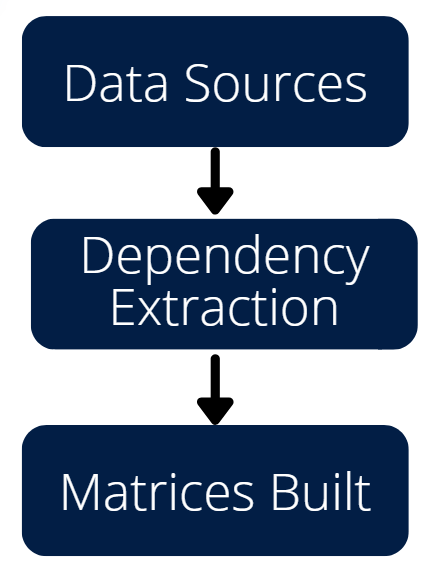
\includegraphics[width=0.9\textwidth]{Imagens/Fluxograma.png}
\end{center}
\end{columns}

\end{frame}

\begin{frame}
\frametitle{Problem Formulation: Multi-Objective Optimization}

\begin{columns}[T]
\column{0.6\textwidth}
\begin{itemize}
\item Recommend a subset $S$ of Python libraries optimizing multiple criteria
\item \textbf{Three competing objectives:}
  \begin{itemize}
  \item \textbf{Maximize Linked Usage (LU):} Co-occurrence in real projects
  \item \textbf{Maximize Weighted Semantic Similarity (SS):} Topical coherence 
  \item \textbf{Minimize Set Size (RSS):} Keep recommendations concise
  \end{itemize}
\end{itemize}

\column{0.4\textwidth}
\begin{center}
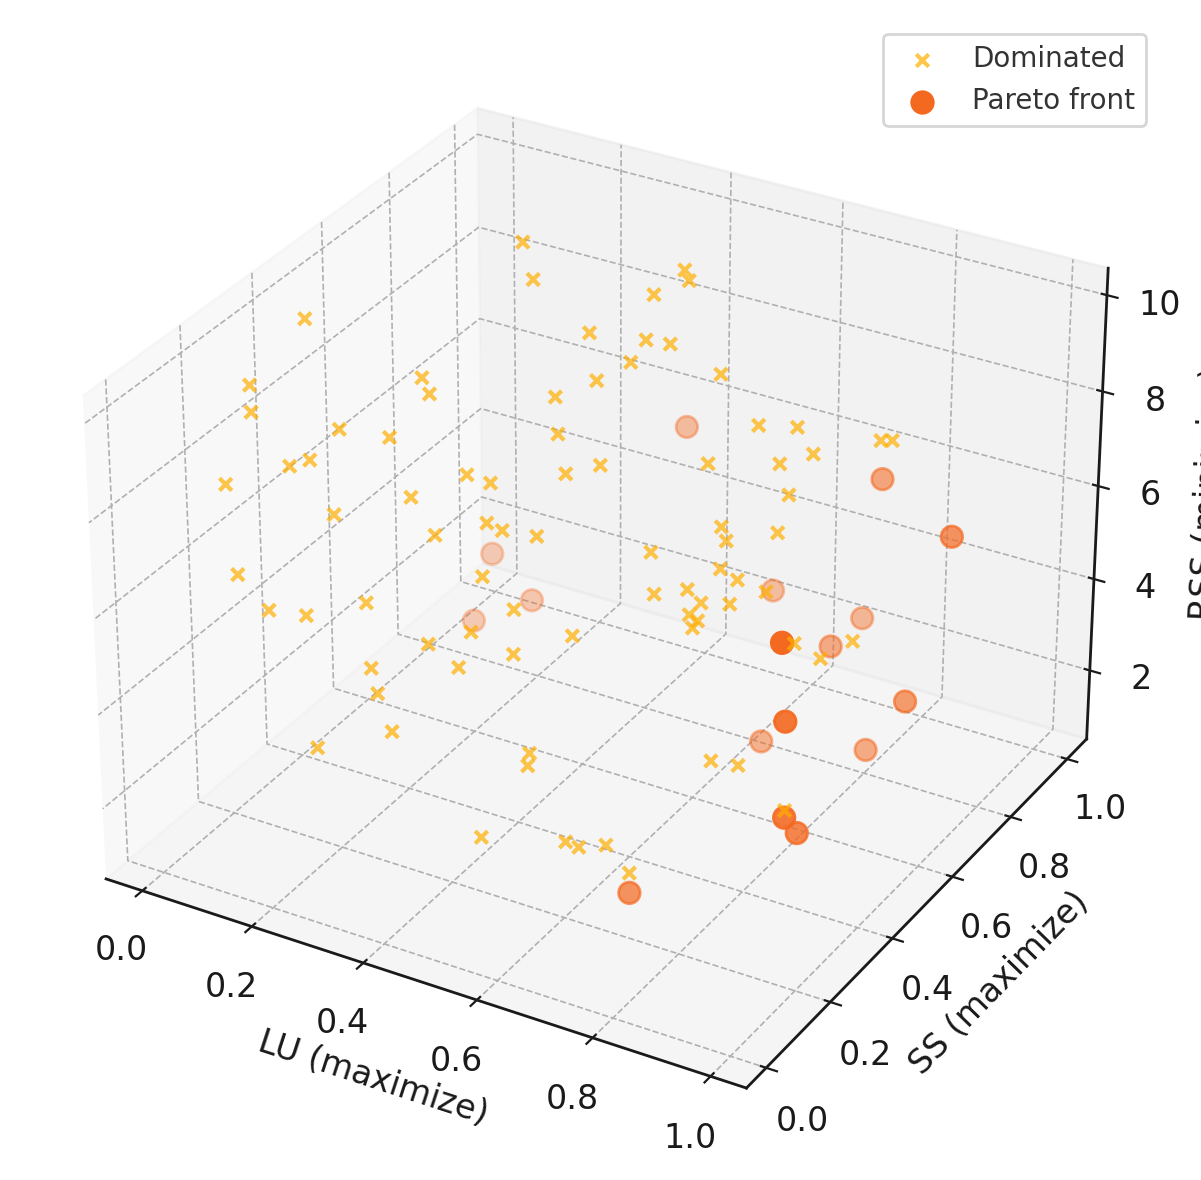
\includegraphics[width=0.9\textwidth]{Imagens/Non-Dominated_Solutions.png}
\captionof{figure}{Non-Dominated Solutions}
\end{center}
\end{columns}
\end{frame}

\begin{frame}
\frametitle{Multi-Objective VNS Framework}

\begin{columns}[T]
\column{0.8\textwidth}
\begin{itemize}
\item \textbf{Solution representation:} Binary vector encoding
\item \textbf{VNS advantages:}
  \begin{itemize}
  \item Systematic neighborhood exploration
  \item Effective for combinatorial spaces
  \item Superior to GA for subset selection problems
  \end{itemize}
\item \textbf{Core algorithm:}
  \begin{itemize}
  \item Initial solution → Pareto local search
  \item Systematic neighborhood changes (intensification)
  \item Shaking for escaping local optima (diversification)
  \end{itemize}
\end{itemize}


\end{columns}
\end{frame}

\begin{frame}
\frametitle{Neighborhood Structures for Library Selection}

\begin{columns}[T]
\column{0.58\textwidth}
\vspace{1.5cm}
\textbf{Tailored neighborhoods for subset selection:}
\begin{itemize}
\item \textbf{N$_1$ (Addition):} Add one library
  \begin{itemize}
  \item N$_1$(S) = \{S $\cup$ \{$\ell$\} : $\ell$ $\in$ U$\setminus$(S$\cup$X)\}
  \end{itemize}
\item \textbf{N$_2$ (Removal):} Remove one library
  \begin{itemize}
  \item N$_2$(S) = \{S $\setminus$ \{$\ell$\} : $\ell$ $\in$ S, |S| > 1\}
  \end{itemize}
\item \textbf{N$_3$ (Swap):} Replace one library
  \begin{itemize}
  \item Maintains size while improving solution quality
  \end{itemize}
\end{itemize}
\column{0.42\textwidth}
\begin{center}
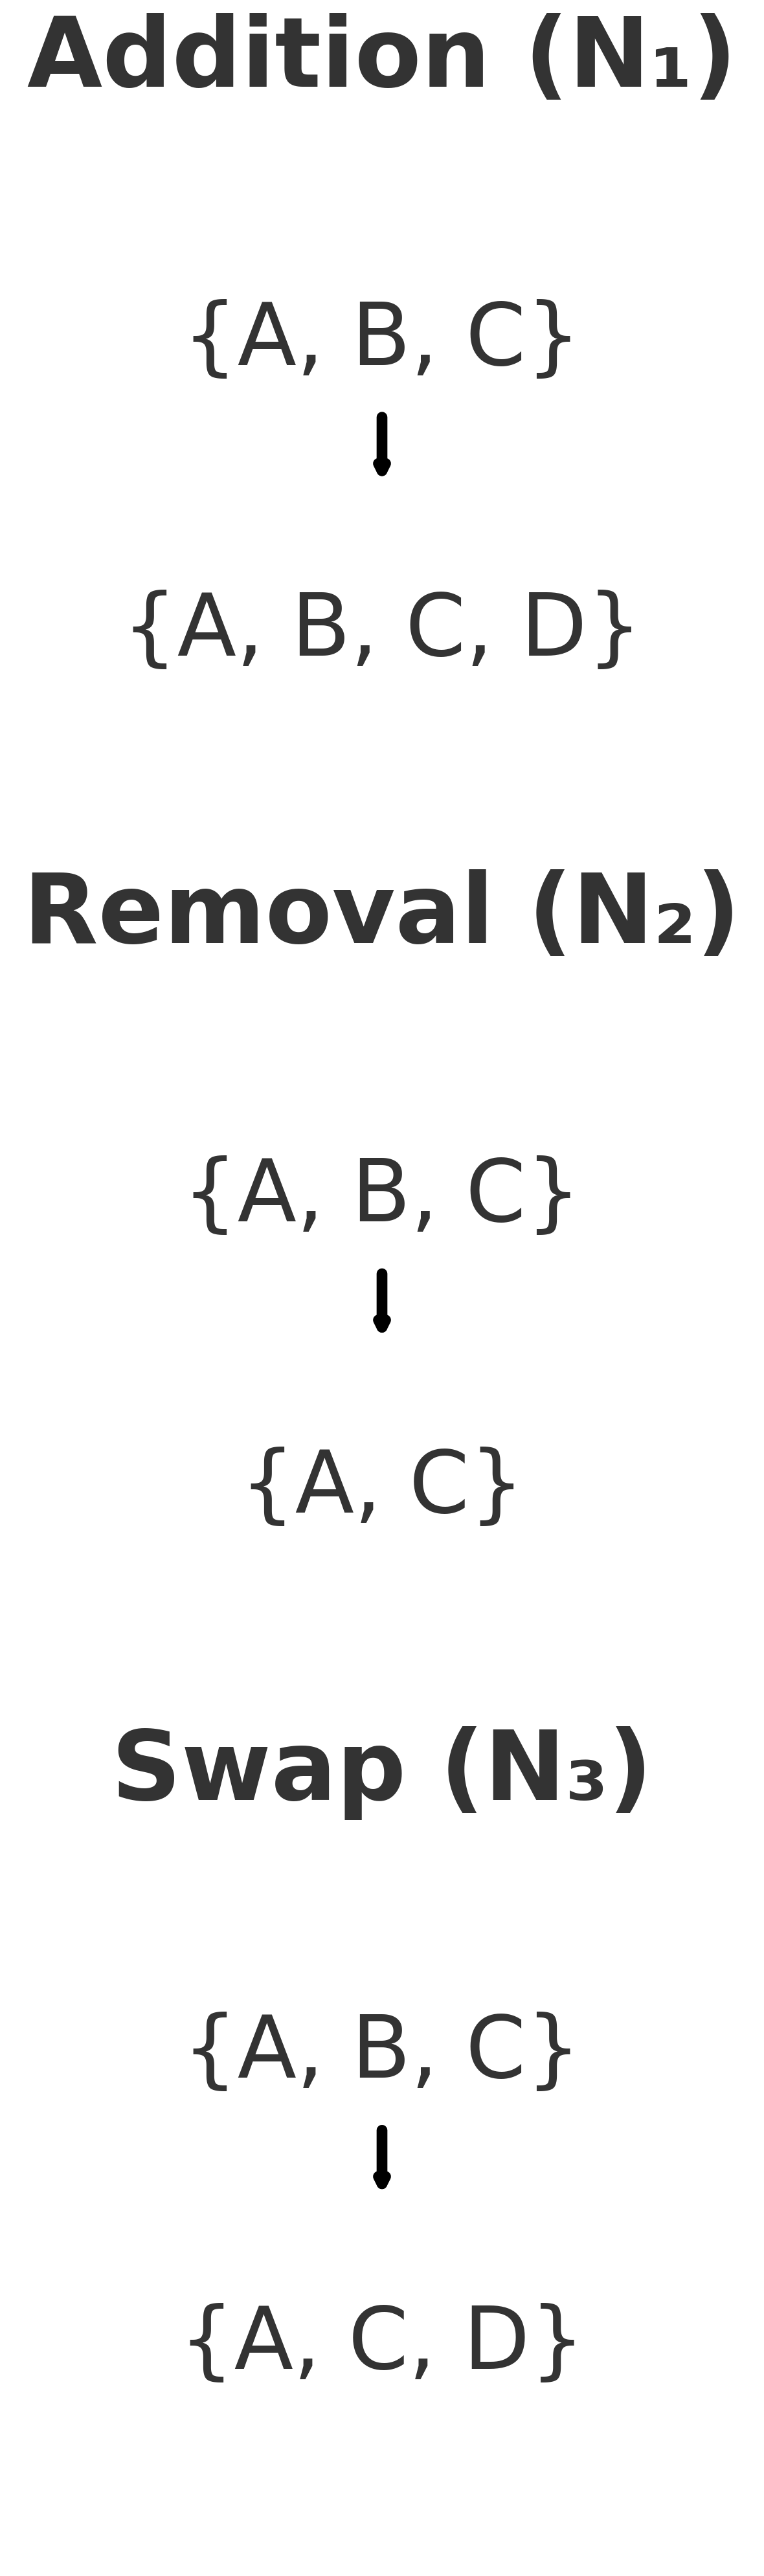
\includegraphics[width=0.4\textwidth]{Imagens/Operaçoes_vizinhaça.png}
%\captionof{figure}{Neighborhood moves}
\end{center}
\end{columns}
\end{frame}

\begin{frame}
\frametitle{Pareto Archive \& Performance Metrics}

\begin{itemize}
\item \textbf{Elite Archive $\mathcal{A}$} stores all non-dominated solutions
\vspace{0.2cm}
  \begin{itemize}
  \item Add new solution if non-dominated
  \item Remove any dominated solutions
  \item Guarantees non-decreasing hypervolume
  \end{itemize}
  \vspace{0.2cm}
\item \textbf{Key performance indicators:}
\vspace{0.2cm}
\begin{itemize}
  \item \textbf{Hypervolume (HV):} Measures convergence and diversity
  \item \textbf{Spread ($\Delta$):} Distribution uniformity across Pareto front
  \item \textbf{$\varepsilon$-indicator:} Convergence between iterations
\end{itemize}
\end{itemize}

\end{frame}

\begin{frame}
\frametitle{Experimental Setup}
\begin{columns}[T]
\column{0.95\textwidth}
\begin{itemize}
\item \textbf{Benchmarks:}
  \begin{itemize}
  \item 10 context libraries (scikit-learn, XGBoost, etc.)
  \end{itemize}
\item \textbf{Algorithm parameters:}
  \begin{itemize}
  \item NSGA-II: Pop=200, generations=500, crossover=0.9, mutation=0.1
  \item MOVNS: 3 neighborhoods, archive size=100, shake strength=3-7
  \end{itemize}
\item \textbf{Evaluation:}
  \begin{itemize}
  \item Computational budget: 2 minutes
  \item Metrics: Hypervolume, Spread ($\Delta$), $\varepsilon$-indicator
  \end{itemize}
\end{itemize}
\end{columns}
\end{frame}

\begin{frame}
\frametitle{Convergence Results}

%\begin{columns}[T]
%\column{0.58\textwidth}
\begin{center}
\begin{tabular}{lrr}
\toprule
\textbf{Metric} & \textbf{NSGA2} & \textbf{MOVNS} \\
\midrule
Final HV & 0.712 & \textbf{0.748} \\
$\epsilon$-indicator & 0.087 & \textbf{0.062} \\
time(s) & \textbf{ 8s }  & \textbf{ 7s }\\ 
\bottomrule
\end{tabular}
\end{center}
\vspace{0.5cm}
\begin{center}
\begin{itemize}
\item MOVNS: 5.1\% higher hypervolume
\item 15.2\% faster early convergence
\item Better $\epsilon$-indicator
\end{itemize}
\end{center}

%\column{0.42\textwidth}
%\begin{center}
%\includegraphics[width=0.92\textwidth]{convergence_chart.png}
%\end{center}
%\end{columns}
\end{frame}



\begin{frame}
\frametitle{PyCommend VNS Results: Context Libraries}

\begin{columns}[T]
\column{0.95\textwidth}
\textbf{Test Case Inputs:}
\begin{itemize}
\item \textbf{Pyomo}: Optimization modeling language (1.2k)
\item \textbf{FastAPI}: Modern web framework (65k)
\item \textbf{Prophet}: Time series forecasting (16.1k)
\item \textbf{scikit-learn}: ML library for Python (55k)
\item \textbf{pandas}: Data analysis toolkit (38.2k)
\item \textbf{OR-Tools}: Google's optimization suite 
\item \textbf{XGBoost}: Gradient boosting 
\end{itemize}

\vspace{0.1cm}
\textbf{Input library characteristics:}
\begin{itemize}
\item Libraries spanning data science, ML, web, and optimization domains
\item Range from established frameworks to specialized tools
\end{itemize}
\end{columns}
\end{frame}


\begin{frame}
\frametitle{PyCommend VNS Results: Recommendations}

\begin{columns}[T]
\column{0.95\textwidth}
\textbf{Pareto-optimal recommendations} 
\begingroup
\footnotesize
\begin{table}[h]
\centering
\setlength{\tabcolsep}{4pt}
\begin{tabular}{p{1.7cm}p{8.5cm}c}
\toprule
\textbf{Input} & \textbf{Recommended Set} & \textbf{Size} \\
\midrule
FastAPI & pydantic, uvicorn, typer & 3 \\
FastAPI & pydantic, uvicorn, starlette, httpx, pytest, jinja2, SQLAlchemy & 7 \\
OR-Tools & DEAP, pymoo,  Minizinc & 4 \\
OR-Tools & DEAP, Minizinc, pulp, pygad & 4 \\
Prophet & pandas, matplotlib, numpy, scikit-learn & 4 \\
Pyomo & pymoo, numpy, scipy, networkx & 4 \\
Pyomo & pymoo, numpy, scipy, pandas, matplotlib, networkx & 6 \\
Ray & tune, numpy & 2 \\
Ray & tune, numpy, pandas, dask, modin, prefect, mlflow & 7 \\
scikit-learn & Optuna, XGBoost, joblib & 3 \\
scikit-learn & pandas, matplotlib, seaborn, XGBoost, joblib, yellowbrick & 6 \\
XGBoost & Optuna, pandas, numpy & 3 \\
XGBoost & Optuna, pandas, numpy, scikit-learn, mlflow & 5 \\
\bottomrule
\end{tabular}
\end{table}
\endgroup
\end{columns}
\end{frame}

\begin{frame}
\frametitle{PyCommend VNS Results: Ecosystem Patterns}

\textbf{Real-world library co-occurrence patterns:}
\vspace{0.1cm}
\begin{center}
\begin{tabular}{p{3.2cm}p{7cm}}
\toprule
\textbf{Domain} & \textbf{Common Library Combinations} \\
\midrule
Machine Learning & scikit-learn + XGBoost + Optuna \\
Model Deployment & FastAPI + Pydantic + uvicorn \\
Optimization & Academic: Pyomo + solvers + OR-Tools \\
Time Series & Prophet + Pandas + Matplotlib/Seaborn \\
\bottomrule
\end{tabular}
\end{center}

\small
\vspace{0.2cm}
\textbf{Key ecosystem insights:}
\begin{itemize}
\item \textbf{API Compatibility:} Compatible libraries show strongest co-occurrence
\item \textbf{Workflow Integration:} Complementary functionality drives adoption 
\item \textbf{No Universal Standards:} Ecosystem lacks a hierarquical classification and a compatibility scoring systems
\item \textbf{Domain Specialization:} Clear library preferences exist 
\item \textbf{Validation Methods:} Data mining, dependency checks and community 
\end{itemize}

\end{frame}

\begin{frame}
\frametitle{Conclusions \& Future Work}

\begin{columns}[T]
\column{0.5\textwidth}
\textbf{Conclusions:}
\begin{itemize}
\item The MOVNS framework efficiently recommends diverse and novel library sets with minimal computational overhead.
\item Multi-objective approach balances usage patterns, semantic similarity, and conciseness
\item Real-world ecosystem patterns validate recommendation quality
\item Library co-occurrence reflects both technical compatibility and workflow optimization
\end{itemize}

\column{0.5\textwidth}
\textbf{Future Work:}
\begin{itemize}
\item Security considerations in library recommendations
\item Version compatibility between recommended libraries
\item License compatibility analysis for production use
\item Expansion to other programming languages (C++)
\item Repository and datasets will be publicly available after publication
\end{itemize}
\end{columns}

\end{frame}

\begin{frame}{Acknowledgments}
    \begin{center}
        \large
        {augustompm@id.uff.br - linkedin.com/in/msc-augusto-m}\\[0.2cm]
        {filipe.sousa@pos.ime.uerj.br}\\[0.2cm]
        %\\[0.5cm]
        \small Thanks for the support of Brazilian funding agencies FAPERJ, CAPES and CNPq\\
        \Huge{Thank you!}\\[1cm]
        \large
        Special thanks to:\\
        The ICVNS-2025 Organizing Committee\\
        Professor Daniel Aloise %[0.2cm]

        % Images side by side

        
\includegraphics[height=1.5cm]{faperj.png}
        %\large         
    \end{center}
\end{frame}

\end{document}
